\documentclass[a4paper,11pt,notitlepage]{report}
% Henrik Lund Kramsh�j, February 2001 
% hlk@security6.net,
% My standard packages 
\usepackage{solido-network-exercises}

\begin{document}

\selectlanguage{english}

\newcommand{\emne}[1]{hacker workshop} 
\newcommand{\kursus}[1]{ethical hacker workshop}
\newcommand{\kursusnavn}[1]{ethical hacker workshop\\ exercises}



\mytitle{Ethical Hacker Workshop}{exercises}


\pagenumbering{roman}
\setlength{\parskip}{0pt}

\setcounter{tocdepth}{0}

\normal

{\color{titlecolor}\tableofcontents}
%\listoffigures - not used
%\listoftables - not used 

\normal
\pagestyle{fancyplain}
\chapter*{\color{titlecolor}Preface}
\markboth{Preface}{}
This material is prepared for use in \emph{\kursus} and was prepared by
Henrik Lund Kramsh�j, \link{http://www.security6.net}

This materiale is expected to describe networking setup and
applications for trainings and workshops where hands-on exercises are needed.

Further a presentation is used which is handed out and some other documents that can assist during exercises.

\vskip 1cm
Have fun and learn
%\eject

\section*{\color{titlecolor}Overview}
\markright{Overview}
\setlength{\parskip}{10pt}

This material has some degree of freedom with regards to setup of the environment.

The purpose is to give participants a feel for practical setups. The suggested configurations
and applications are close to real life scenarios but have been designed to fit in with existing infrastructures used for training.


\section*{\color{titlecolor}Prerequisites}

This material expect that participants have a working knowledge of
TCP/IP from a user perspective. Basic concepts such as web site addresses and email should be known as well as IP-addresses and common protocols like DHCP.

\section*{\color{titlecolor}Tools used}
%\markright{V�rkt�jer}

These exercises are expected to be performed in a training setting with network connected workstations.

The exercises use a number of tools which can be copied and reused after training.

Tools used are mostly:

\begin{itemize}
\item Unix - such as Linux, OpenBSD, NetBSD, FreeBSD or Mac OS X
\item Microsoft Windows - primary use is for workstations
\item The requirements for the workstations are a browser and Secure Shell Access
\item In most trainings a Linux based security tool is distributed which is called BackTrack. This tool can be used as a live CD or installed to hard disk.
\end{itemize}


% =================== body of the document ===============
% Arabic page numbers
\pagenumbering{arabic}
\rhead{\fancyplain{}{\bf \chaptername\ \thechapter}}

% Main chapters
%---------------------------------------------------------------------
% gennemgang af emnet
% check questions
% eventuelle �bne sp�rgsm�l
% henvisning til �velse, hvis der er en 

\chapter*{\color{titlecolor}Introduction to networking}
%\markboth{Introduktion til netv�rk}{}
\label{chap:intro}

\section*{\color{titlecolor}IP - Internet protocol suite}

It is extremely important to have a working knowledge about IP to implement
secure and robust infrastructures. Knowing about the alternatives while doing 
implementation will allow the selection of the best features.

\section*{\color{titlecolor}ISO/OSI reference model}
A very famous model used for describing networking is the ISO/OSI model
of networking which describes layering of network protocols in stacks.

This model divides the problem of communicating into layers which can
then solve the problem as smaller individual problems and the solution 
later combined to provide networking.

Having layering has proven also in real life to be helpful, for instance 
replacing older hardware technologies with new and more efficient technologies
without changing the upper layers.

In the picture the OSI reference model is shown along side with 
the Internet Protocol suite model which can also be considered to have different layers.


\begin{figure}[H]
\label{fig:osi}
\begin{center}
\colorbox{white}{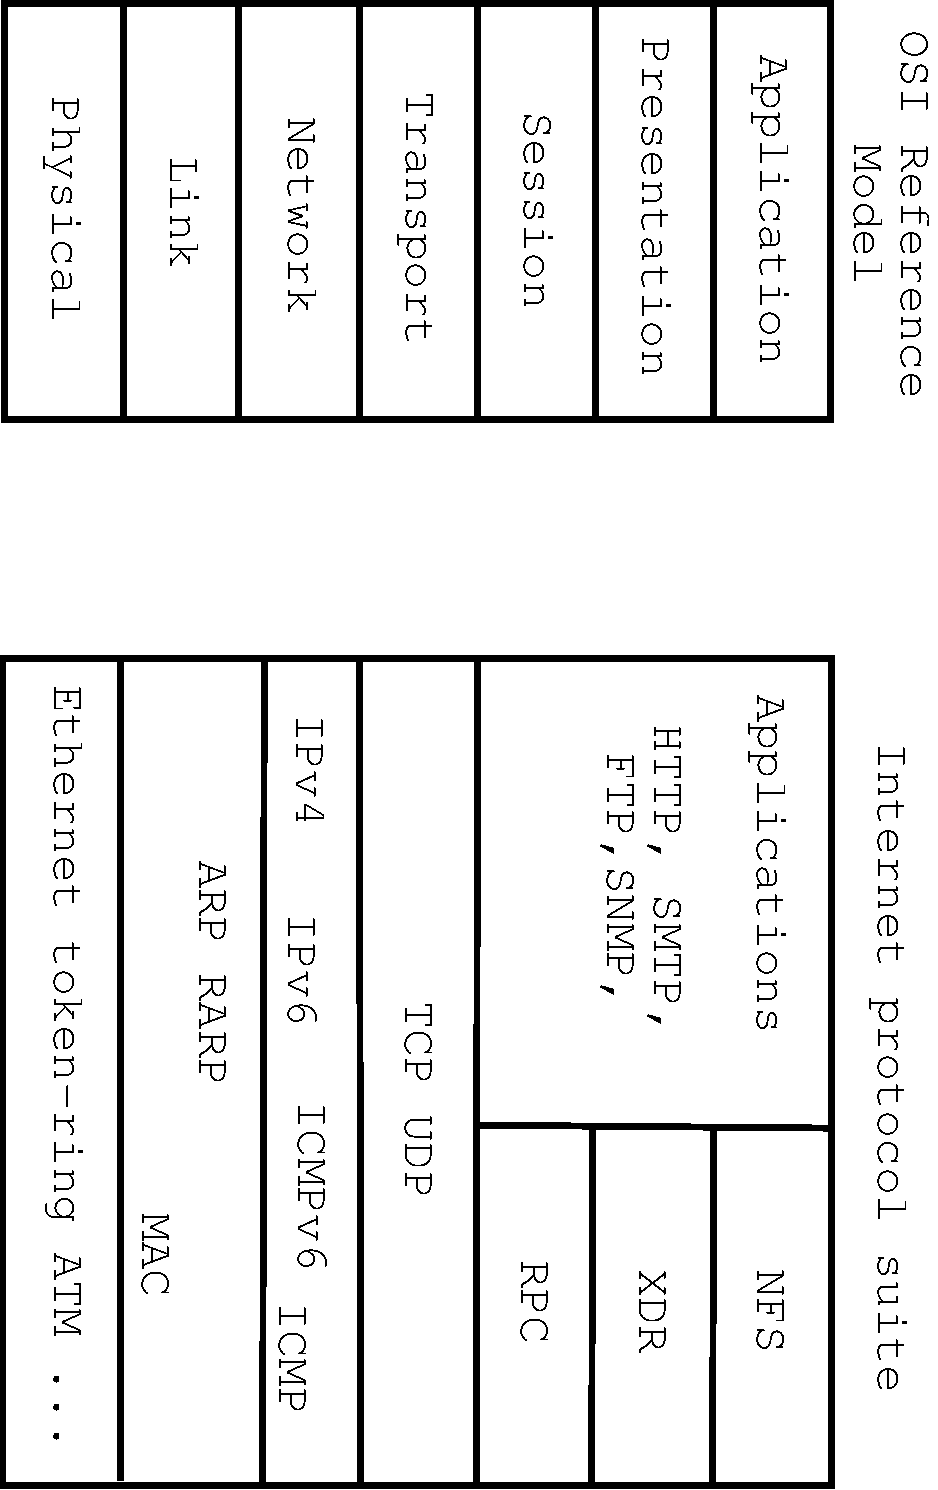
\includegraphics[width=8cm,angle=90]{images/compare-osi-ip.pdf}}
\end{center}
\caption{OSI og Internet Protocol suite}
\end{figure}


\section*{\color{titlecolor}Standards and RFC}

The internet has a number of working groups which are tasked with describing
new features and protocols considered for use on the internet. These 
working groups primarily function across the internet using open mailing lists
in which anyone can contribute to discussion.

When consensus is reached the features are described in document which
are named Request For Comments, or RFC for short. These documents can 
be obtained free of charge from their web site\\ \link{http://www.rfc-editor.org/}. 

Some RFC documents describe actual standards or specific uses and are noted in various
indexing documents called standards (STD), For Your Information (FYI) and Best
Current Practice (BCP).

Whenever a standard is to be updated a new RFC is published and the old version
is not changed allowing the RFC series to also document the development of
the internet standards from the oldest documents in the 1969.

One example is the IP specification itself (IPv4) from 1981:\\
0791 Internet Protocol. J. Postel. Sep-01-1981. (Format: TXT=97779
bytes) (Obsoletes RFC0760) (Updated by RFC1349) (Also STD0005)
(Status: STANDARD) 

As specified the document RFC-0791 is a standard and it was superseeded
by the new verson which is RFC-1349 - which was in fact also updated by 
other documents.


\section*{\color{titlecolor}Adressing in the network}

The network is expected to use private IP-addresses, which are specified in 
RFC-1918 \emph{Address Allocation for Private Internets}

The default subnet to use is:
\begin{itemize}
\item 10.0.45.0/24 - which is about 250 addresses in a subnet with 24 mask bits
\end{itemize}

If internet connectivity is needed and available it will be connected through
a router leaving us with an isolated subnet which can be used for various experiments.


\chapter*{\color{titlecolor}Hardware and networking used}
%\markboth{Hardware og netv�rk til �velserne}{}

This chapter describes the required hardware and software
used for doing exercises.

The requisites should be similar to what is found in a normal setting with
PCs running Microsoft Windows clients and having basic network connectivity.

Parts of the exercises are using Unix, specifically OpenBSD and Linux. Unix
is provided and no prior knowledge of Unix is expected.

A number of programs to be used on Microsoft Windows are provided using
a web server:
\begin{itemize}
\item Putty - SSH access from Microsoft Windows
\item Winscp - easy access to the filesystem on the Unix server using SSH
and also has a built-in editor
\item Wireshark - an open source network protocol analyzer
\end{itemize}


\chapter*{\color{titlecolor}Exercise content}
\markboth{Exercise content}{}

Most exercises follow the same procedure and has the following content:
\begin{itemize}
\item {\bf Objective:} What is the exercise about, the objective
\item {\bf Purpose:} What is to be the expected outcome and goal of doing this exercise
\item {\bf Suggested method:} suggest a way to get started
\item {\bf Hints:} one or more hints and tips or even description how to 
do the actual exercises
\item {\bf Solution:} one possible solution is specified 
\item {\bf Discussion:} Further things to note about the exercises, things to remember and discuss
\end{itemize}

Please note that the method and contents are similar to real life scenarios and does not detail every step of doing the exercises. Entering commands directly from a book only teaches typing, while the exercises are designed to help you become able to learn and actually research solutions.



\chapter{Putty installation - Secure Shell login}
\label{ex:putty-install}
\hlkimage{6cm}{images/putty-1.jpg}

{\bf Objective:}\\
Install the program Putty locally on your workstation

{\bf Purpose:}\\ 
Installing Putty will make sure you have administrative access and allow us to use Secure Shell for connecting to Unix systems and networking devices.

{\bf Suggested method:}\\
Download and install the program, either download from web server locally or from\\
\url{http://www.chiark.greenend.org.uk/~sgtatham/putty/download.html}


{\bf Hints:}\\ 
Putty is a terminal emulator and replaces the telnet program in Windows.
It is often the preferred way of connecting to Unix systems and is also 
available in network devices such as switches, routers and firewalls.

Further Putty will enable serial connections which can be used for configuring
equipment through console connections. Remember to select the method
when using Putty.

It is suggested to save profiles for future use, and remember to change a 
profile you should load the profile, make changes and {\bf remember to go back
and save the profile} before opening a connection. Otherwise the profiles changes
will only be active in the current connection.

{\bf Solution:}\\
Do a normal installation with default settings. 

If you known Putty already you can investigate the Puttygen program and
research the use of public and private keys.

{\bf Discussion:}\\
The Secure Shell protocol is an internet standard for secure terminal connections
and the same protocol allows file transfer and forwarding of network packets.

Note: the procotol version 2 is the one recommended

\chapter{WinSCP installation - Secure Copy}
\label{ex:winscp-install}

\hlkimage{6cm}{images/winscp-explorer.png} 

{\bf Objective:}\\
Install the program WinSCP locally on your workstation


{\bf Purpose:}\\ 
Get required programs ready for doing exercises.

{\bf Suggested method:}\\ 
Installing WinSCP will make sure you have access to transferring files from Unix systems and networking devices.


{\bf Hints:}\\
WinSCP is very helpful allowing easy access to files using Secure Shell protocol
and also when working with text files it is possible to use the built-in editor 
of WinSCP.

{\bf Solution:}\\
Download and install the program

{\bf Discussion:}\\ 
WinSCP can also be used instead of FTP, why is that helpful?

\chapter{Login to Unix server}
\label{ex:unix-login}

\hlkimage{6cm}{images/putty-screen2.jpg}

{\bf Objective:}\\
Do a remote login from your workstation to the servers provided

{\bf Purpose:}\\ 
Make sure the network is working and allow you to use the Unix system for exercises.

{\bf Suggested method:}\\
You will use Putty or another Secure Shell program and login to the servers provided

{\bf Hints:}\\
Use the Putty program or boot the Linux Live CD and run ssh from the command line.

Using the Linux Live CD the OpenSSH programs are already installed and available
and are used with commands like this::\\
\verb+ssh username@server -p port+ which for the actual server is:\\
\verb+ssh team1@10.0.45.45 -p 22+

NB: the server may have another IP-address due to the use of DHCP

The users defined all have the password {\bf team}

{\bf Solution:}\\
Start Putty or boot using the Linux Live CD 

{\bf Discussion:}\\
The Linux Live CD is based on Open Source and may be copied freely.

The BackTrack security distribution contain more than 300 security programs and is being updated actively.


\chapter{Get to know some Unix}
\label{ex:unix-cal}
%\hlkimage{6cm}{images/putty-1.jpg}

{\bf Objective:}\\
Try a few Unix commands and see that help is available

Answer the following questions:
\begin{itemize}
\item What does the command \verb+cal+ do? What happened in September 1752?
\item What does the commands \verb+date+, \verb+clear+ and \verb+echo+ do?
\end{itemize}

{\bf Purpose:}\\
Learn enough Unix to be able to run simple commands from the command line 

{\bf Suggested method:}\\ 
Log into the Unix system and try executing the commands

After trying the commands use the manual pages with the following commands:\\
\verb+man cal+, \verb+man date+, \verb+man clear+,
\verb+man echo+

\begin{alltt}
$ date
...
$ cal
...
$ cal 2009
...
$ cal 1752
... 
output is not shown on purpose, try it for yourselves :-)
\end{alltt}

{\bf Hints:}\\
The manual system is always available on Unix and usually you can do searches when
displaying a manual page using the operators / (forward search) and ? (backward search).

{\bf Solution:}\\
Type \verb+man cal+ and do a search by entering /, the year 1752 and press enter

{\bf Discussion:}\\
Searching using / and ? are very common on Unix 


\chapter{Access the root on Unix}
\label{ex:sudo}
%\hlkimage{6cm}{images/putty-1.jpg}

{\bf Objective:}\\
Learn to use the sudo command to gain root access.

{\bf Purpose:}\\
Know a way to gain access as root user - to run hacker programs later

{\bf Suggested method:}\\ 
Run the command and use the manuals of the two commands \verb+su+ and \verb+sudo+
to answer the following questions:
\begin{itemize}
\item What is the goal of the progams?
\item What are the similarities and differences?
\item Can the su command be configured not to use a password? can sudo?
\item What password needs to be entered when using the programms, your pasword or the superuser password?
\end{itemize}

{\bf Hints:}\\
Switch user is the old command used to gain root access - and requires the knowledge of the password for the root user or the other user your are switching to. Su always give complete access by switching to the user id. Sudo is a more modern way to control access.

{\bf Solution:}\\
Use the command \verb+sudo -s+ to get root access and then exit to exit superuser.

{\bf Discussion:}\\
Unix systems have traditionally used the switch user \verb+su -+ but the superuser do
\verb+sudo+ is much more modern and flexible by allowing you to specify specific commands and permissions
on a fine grained permission model. 

Sudo is used almost exclusively and is considered the de facto way of gaining root on Unix systems.

An example use of sudo might be the restarting of a web server with apache control:
\begin{alltt}    
\small
hlk@bigfoot:hlk$ sudo apachectl configtest
Syntax OK
hlk@bigfoot:hlk$ sudo apachectl restart    
hlk@bigfoot:hlk$ 
\end{alltt}
(Note: when things succeed Unix wont say much, only if something unexpected happens there will be output)


\chapter{Unix boot CD}
\label{ex:unix-boot-cd}
\hlkimage{8cm}{backtrack4-logo.png}

{\bf Objective:}\\
Boot a Live CD on the workstation

{\bf Purpose:}\\
Learn to use Live CD's - specifically the BackTrack Live CD

{\bf Suggested method:}\\ 
Insert the DVD and boot from it

{\bf Hints:}\\
There is a large number of Live CDs built on the Linux operating system
specifically designed for various purposes. Some of the well known CDs are:

\begin{itemize}
\item Knoppix which include a lot of productivity tools, like web browser,
office suite, mail programs etc.
\item BackTrack which include more than 300 security tools and a premade Linux kernel with a lot of security related patches.
\item Damn Vulnerable Linux which is also a security CD but the focus is on providing a learning evironment for security training. Some tools help work with buffer overflows and others provide an opportunity to do reverse engineering
\end{itemize}

{\bf Solution:}\\
When booted use the commands shown below

{\bf Discussion:}\\
The Live CDs are designed to be used on most computer, but some models
require more work - typically the graphic card or wireless network card can cause trouble.

If that should happen it is recommended to search on the internet, to see if others have tried using Linux on the specific brand and model of computer.

In case of the wireless card not working it is recommended to research and buy
a wireless network card that is known to work.

{\bf Note: When working with the BackTrack CD the following commands are usefull:}
\begin{itemize}
\item \verb+startx+ will enter the graphical environment
\item \verb+/etc/init.d/networking start+ will try configuring the network on all interfaces with DHCP
\item \verb+dhclient eth0+ start a single DHCP client using a specific network card, like eth0
\item \verb+wicd+ followed by \verb+wicd-client+ will start a wireless client program to allow you to join wireless networks
\item \verb+apt-get update+ and \verb+apt-get upgrade+ - upgrade when installed in hard disk
\item \verb+apt-get update+ and \verb+apt-get dist-upgrade+ - upgrade with major upgrades
\end{itemize}

The individual tools on the BackTrack are described in detail on the internet and some of the tools, like Wireshark and nmap will have excellent documentation avaiable.

\chapter{Wireshark installation}
\label{ex:wireshark}

\hlkimage{10cm}{ethereal-main-window.pdf} 


{\bf Objective:}\\
Install the program Wireshark locally on the Windows workstation

{\bf Purpose:}\\
Installing Wireshark will allow you to analyse packets and protocols

{\bf Suggested method:}\\ 
Download and install the program, either download from web server locally or from \link{http://www.wireshark.org}\\
Wireshark requires a Windows Capture library to be installed, which is included in the
Wireshark installation, but can none the less be downloaded from\link{http://www.winpcap.org/}\\

{\bf Hints:}\\ 
PCAP is a packet capture library allowing you to read packets from the network. Wireshark is a graphical application to allow you to browse through traffic, packets and protocols.

{\bf Solution:}\\
When Wireshark is installed sniff some packets, also see next exercise.

{\bf Discussion:}\\ 
Wireshark is just an example other packet analyzers exist, some commercial and some open source like Wireshark

\chapter{Sniffing network packets}
\label{ex:wireshark-sniff}

{\bf Objective:}\\ 
Sniff packets and dissect them using Wireshark

{\bf Purpose:}\\
See real network traffic, also know that a lot of information is available and not encrypted. 

{\bf Suggested method:}\\ 
Open Wireshark and start a capture - either from Windows or BackTrack\\
Then in another window execute the ping program while sniffing

{\bf Hints:}\\
When running on Linux the network cards are named eth0 for the first Ethernet and wlan0 for the first Wireless network card. In Windows the names of the network cards are long and if you cannot see which cards to use then try them one by one.

{\bf Solution:}\\
When you have collected some packets you are done.

{\bf Discussion:} 
Is it ethical to collect packets from an open wireless network?

\chapter{Discovery using ping and traceroute}
\label{ex:ping}

{\bf Objective:}\\ 
Learn how to use the ping and traceroute programs.

{\bf Purpose:}\\
Doing network discovery is an important part of doing security testing.

{\bf Suggested method:} \\
Use \verb+ping+ and \verb+traceroute+ testing your network connection.

Can be performed from both Windows and Unix/Linux

Remember though that traceroute is named \verb+tracert+ on Windows.

{\bf Hints:} \\
ICMP is the Internet Control Message Protocol which is used for reporting problems back to a source on the internet. It can also be used for diagnosing problems using ICMP ECHO request packets. ICMP is very important when doing security testing for network discovery and making sure connections are alive.

The following protocols are being used:
\begin{itemize}
\item Ping uses ICMP packets with request and expect responses
\item Tracert on Windows uses ICMP packets
\item Traceroute on Unix by default uses UDP packets, but can also use ICMP
\end{itemize}

{\bf Solution:}\\
Run the commands - not all are available on Windows, so perhaps use Unix:
\begin{itemize}
\item {\bf traceroute} (Unix) or {\bf tracert} (Windows)
\item {\bf traceroute -I}\\ 
\end{itemize}

{\bf Discussion:}
A lot of people just try to block any ICMP, but that will actually hurt a lot of functionality within your network.

Other trace programs exist, for example TCP traceroute programs - find them on the BackTrack!

\chapter{ICMP tool - icmpush}
\label{ex:icmpush}

{\bf Objective:} \\
See a sample program that allows you to send ICMP packets without doing actual programming

{\bf Purpose:}\\ 
Know that a lot of hacker programs exist on any level of IP

{\bf Suggested method:} \\
Login to the Unix server - see the manual and use timestamp request packets

Alternative install icmpush on BackTrack using the command apt-get, try running icmpush and
then follow on screen instructions.

{\bf Hints:} \\

{\bf Solution:}\\
Use the command \verb+icmpush -v -tstamp 10.0.45.45+
and also try echo, mask from the icmpush program

{\bf Discussion:}\\ 
Other toolboxes for creating network packets are:
\begin{itemize}
\item Nemesis - which is on the BackTrack
\item Scapy - which allow you to do Python programs that can send packets
\item Hping - which is on the BackTrack
\end{itemize}

\chapter{Lookup Whois data}
\label{ex:whois}


{\bf Objective:} \\
Learn to use Whois databases

{\bf Purpose:}\\ 
Knowing who to contact in case of problems on the internet is important, and also verifying before starting scanning is required.

{\bf Suggested method:}\\
\begin{itemize}
\item Login to the UNIX server and use \verb+whois+ or use the web interfaces
like \\ \link{http://www.ripe.net}
\end{itemize}

{\bf Hints:}\\ 
Whois databases are distributed to Regional Internet Registries such as ARIN, AfriNIC, RIPE, LACNIC and APNIC.

{\bf Solution:}\\
Use the specified command above with an IP address, \verb+whois 91.102.91.17+.

{\bf Discussion:}\\
The whois system was implemented after the Morris Worm affected the internet in November 1988, because it was realized that the internet had grown to a size that required more management.


\chapter{Discover using DNS}
\label{ex:basic-dns-lookup}

{\bf Objective:}\\
Try some programs for doing Domain Name System (DNS) lookups

{\bf Purpose:}\\ 
Learning to do network discovery includes looking into public information such as DNS

{\bf Suggested method:}\\

Try these commands:
\begin{itemize}
\item nslookup - available on both Unix and Windows, but not recommended anymore
\item Try \verb+nslookup -q=txt -class=CHAOS version.bind. 0+  
\item Try \verb+dig @ns1.gratisdns.dk www.security6.net A+
\item Try \verb+host -a security6.net+ and 
\verb+host -a www.security6.net+ any difference? 
\\
\item The host program uses the syntax \verb+host host server+ while dig uses \verb+dig @server host+
\end{itemize}

{\bf Hints:}\\ 
Host is available by default on OpenBSD, so use the Unix server provided

There are a lot of Graphical User Interface programs available both for Unix and Windows

{\bf Solution:}\\
Run the commands above, output would be like this:

\begin{alltt}
$ host -t ns security6.net
security6.net name server ns1.gratisdns.dk.
security6.net name server ns2.gratisdns.dk.
security6.net name server ns3.gratisdns.dk.
security6.net name server ns4.gratisdns.dk.
security6.net name server ns5.gratisdns.dk.
$ host -t ns security6.net 217.157.20.131
...
\end{alltt}


{\bf Discussion:}\\
Previously it was possible to do Zone Transfers, but today most DNS syste administrators do not allow that. If possible a zone transfer will reveal all names for a domain.

Make sure that you know the difference between forward and reverse lookups. Forward is from name to IP address lookup, while reverse does a lookup from IP address to name.


\chapter{Try the bind-version shell script}
\label{ex:bind-version-script}

{\bf Objective:} 
Try to use a shell script to automate lookups

{\bf Purpose:}\\
When doing actual security testing you should automate as much as possible.

{\bf Suggested method:} 
Login to the Unix server provided and run the bind-version script

{\bf Hints:} 
Unix files with \verb+#!+ as the first line will be executed using the command specified.

Unix shell scripting is very usefull and the book
\emph{Classic shellscripting} is recommended when doing shell scripting.

Unix also typically include scripting languages like Perl, Python, Ruby, Groovy, ...

{\bf Solution:}\\
Run the script provided

{\bf Discussion:} 
The script only does a few DNS lookups, but more elaborate scripts are being used daily by administrators, security consultants and hackers.

The script available on the system is:
{\small
\VerbatimInput{scripts/bindversion}
}


\chapter{Try the dns-timecheck Perl program}
\label{ex:dns-timecheck}

{\bf Objective:} 
Try to use a Perl script to communicate with a binary protocol

{\bf Purpose:}\\ 
See that programming languages such as Perl often include a lot of libraries which allow efficient implementation of ideas.

{\bf Suggested method:} 
Login to the Unix server provided and run the dns-timecheck script

{\bf Hints:} 
Perl can be a bit difficult to read, but a lot of tutorials exist

{\bf Solution:}\\

{\bf Discussion:} 
While Perl has been around for lots of years it seems that security tools are often implemented using these languages:
\begin{itemize}
\item Perl, of course :-)
\item Python - like Scapy
\item Ruby - like Metasploit
\end{itemize}

The script available on the system is:
{\small
\VerbatimInput{scripts/dnstimecheck}
}


\chapter{Research arpspoof and dsniff}
\label{ex:arpspoof}
{\bf Objective:} \\
Read about arpspoof and dsniff

{\bf Purpose:}\\ 
Realize that having a switch does not prevent sniffing, but makes it a bit more difficult.

{\bf Suggested method:} \\
Log onto the Unix server and look at manual pages

{\bf Hints:} \\
ARP spoofing is about sending false information to systems trying to communicate. If it happens the systems will send their packets to the wrong destination, the hacker who can then sniff data and forward. 

Dsniff is a program that can decode a lot of older protocols.

{\bf Solution:}\\
To read manual pages use: \verb+man arpspoof+ and
\verb+man dsniff+


{\bf Discussion:}\\ 
What can be done using these programs?

Please notice that it can make the network a bit unstable if you are not carefull. Luckily the network will recover by itself in 5-10 minutes.

A graphical tool is available on the BackTrack named Ettercap.


\chapter{Discover active systems ping sweep}
\label{ex:nmap-pingsweep}
\hlkimage{10cm}{nmap-zenmap.png}

{\bf Objective:}\\ 
Use nmap to discover active systems

{\bf Purpose:}\\ 
Know how to use nmap to scan networks for active systems.

{\bf Suggested method:}\\ 
Try different scans,
\begin{itemize}
\item Ping sweep to find active systems
\item Port sweeps to find active systems with specific ports
\end{itemize}

{\bf Hints:} \\
Try nmap in sweep mode

{\bf Solution:}\\
Use the command below as examples:
\begin{itemize}
\item Ping sweep \verb+nmap -sP 10.0.45.*+
\item Port sweeps \verb+nmap -p 80 10.0.45.*+
\end{itemize}

{\bf Discussion:}\\ 

{\bf You can also use the graphical interface to nmap called Zenmap.}


\chapter{Execute nmap TCP and UDP port scan}
\label{ex:nmap-synscan}


{\bf Objective:} \\
Use nmap to discover open ports on active systems

{\bf Purpose:}\\ 
Finding open ports will allow you to find vulnerabilities on these ports.

{\bf Suggested method:}\\ 
Use \verb+nmap -p 1-1024 server+ to scan the first 1024 TCP
ports

Try to use \verb+nmap -sU+ to scan using UDP ports, not really possible if a firewall is in place.

If a firewall blocks ICMP you might need to add \verb+-P0+
or even \verb+-PN+ to make nmap scan even if there are no Ping responses

{\bf Hints:} \\
Sample command: \verb+nmap -P0 -sU -p1-1024 server+ UDP port scanning
1024 ports without doing a Ping first

{\bf Solution:}\\
Discover some active systems and you are done.

{\bf Discussion:}\\ 
There is a lot of documentation about the nmap portscanner, even a book by the author
of nmap. Make sure to visit \link{http://www.nmap.org}

TCP and UDP is very different when scanning. TCP is connection/flow oriented and requires a handshake which is very easy to identify. UDP does not have a handshake and most applications will not respond to probes from nmap. If there is no firewall the operating system will respond to UDP probes on closed ports - and the ones that do not respond must be open.

When doing UDP scan on the internet you will almost never get a response, so you cannot tell open (not responding services) from blocked ports (firewall drop packets). Instead try using specific service programs for the services, sample program could be \verb+nsping+ which sends DNS packets, and will often get a response from a DNS server running on UDP port 53.

\chapter{Perform nmap OS detection}
\label{ex:nmap-os}

{\bf Objective:} \\
Use nmap OS detection and see if you can guess the devices on the network

{\bf Purpose:}\\ 
Getting the operating system of a system will allow you to focus your next attacks.

{\bf Suggested method:}\\ 
Look at the list of active systems, or do a ping sweep.

Then add the OS detection using the option \verb+-O+

{\bf Hints:} \\
Use the manual page

The nmap can send a lot of packets that will get different responses, depending on the operating system.

{\bf Solution:}\\
Use a command like \verb+nmap -O -p1-100 10.0.45.45+ 

 
{\bf Discussion:}\\ 
nmap OS detection is not a full proof way of knowing the actual operating system, but in most cases in can detect the family and in some cases it can identify the exact patch level of the system.

Another tool which does the same is Xprobe.

\chapter{Perform nmap service scan}
\label{ex:nmap-service}

{\bf Objective:} \\
Use more advanced features in nmap to discover services.

{\bf Purpose:}\\ 
Getting more intimate with the system will allow more precise discovery of the vulnerabilities and also allow you to select the next tools to run.

{\bf Suggested method:}\\ 
Use \verb+nmap -A+ option for enabling service detection

{\bf Hints:} \\
Look into the manual page of nmap or the web site book about nmap scanning

{\bf Solution:}\\
Run nmap and get results.

{\bf Discussion:}\\ 

Some services will show software versions allowing an attacker easy lookup at web sites to known vulnerabilities and often exploits that will have a high probability of success.

Make sure you know the difference between a vulnerability which is discovered, but not really there, a false positive, and a vulnerability not found due to limitations in the testing tool/method, a false negative.

A sample false positive might be reporting that a Windows server has a vulnerability that you know only to exist in Unix systems.


\chapter{Find systems with SNMP}
\label{ex:find-snmp}

{\bf Objective:}\\ 
Use snmpwalk to research SNMP systems

{\bf Purpose:}\\ 
Learn that gathering information can help an attacker.

{\bf Suggested method:} \\
Log into the Unix server provided and run snmpwalk which is using UDP port 161.

{\bf Hints:} \\
We are running in a LAN environment with less firewalls, so doing nmap UDP scan is possible.

When discovering an IP then use the \verb+snmpwalk+
  program to show a lot of information.


{\bf Solution:}\\
\begin{itemize}
\item Use the command \verb+snmpwalk -v 2c -c public 10.0.45.34 | less +\\
\end{itemize}

The command less will show output one screen at a time.

{\bf Discussion:}\\ 
In real networks SNMP is being used a lot, but new equipment is starting NOT to allow access using the community string public. 

\chapter{Try Hydra brute force}
\label{ex:hydra-brute}

{\bf Objective:}\\ 
Try a brute force program named hydra/Xhydra

{\bf Purpose:}\\ 
Learn that some protocols allow brute forcing.

{\bf Suggested method:} \\
Log into the Unix server or use the BackTrack.

Make a short list of usernames and a short list of passwords 
and use hydra to brute force your way into a system. Use the editor \verb+kate+, using \verb+kate users.txt+ and \verb+kate pass.txt+ followed by a command similar to this:
\begin{alltt}
$ hydra -V -t 1 -L users.txt -P pass.txt 10.0.45.2 ssh
\end{alltt}


{\bf Hints:} \\
When learning tools create a nice environment and check that things are working
before trying to hack. So with brute forcing an account, create and test it!

{\bf Solution:}\\
There is an FTP server with an easy to guess administrator password.

{\bf Discussion:}\\ 
The hydra program can brute force a lot of different protocols and also
allow a lot of tuning. 

The hydra program does an online brute force attack, in some cases you
can get access to data like password databases, or hash values that can
be cracked in off-line brute force attacks.

\chapter{Try Cain brute force}
\label{ex:cain-brute}

\hlkimage{8cm}{cain_brute_attack.png}


{\bf Objective:}\\ 
Try a brute force program named Cain

{\bf Purpose:}\\ 
Learn that some algorithms allow for easier brute forcing.

{\bf Suggested method:} \\
Download and install the Windows program Cain

Then try cracking some local accounts, access to hash is only allowed if you are administrator.

{\bf Hints:} \\
When learning tools create a nice environment and check that things are working
before trying to hack. So with Cain use a system where you are administrator and crack local accounts.

Then later get hash values from real systems, or by doing google searches.

{\bf Solution:}\\
See that some algorithm can do 100.000s keys/second and others only allow 100s keys/second.

{\bf Discussion:}\\ 
Cain is built for cracking passwords in off-line brute force attacks, but also includes other features like sniffing.


\chapter{Network scripting using netcat}
\label{ex:netcat-1}

{\bf Objective:} \\
Learn how to use the netcat program for scripting

{\bf Purpose:}\\ 
Learn that a lot of protocols on the internet are easy read and create tools for.

{\bf Suggested method:} \\
Login to the Unix server - look at the manualen \verb+man nc+.
Then create a textfile named headh.sh using this content
\begin{alltt}
\input{scripts/head.sh}
\end{alltt}

Then use the command \verb#chmod +x head.sh# to make it executable and run it

{\bf Hints:}\\
The netcat program is a swiss army-knife for network data, and allows you to forward data to various ports and connect programs.

{\bf Solution:}\\
Run the program: \verb+./head.sh www.pentest.dk 80+


{\bf Discussion:}\\

Sometime the program will seem to hang, use ctrl-c to break it.

\chapter{OpenSSL forbindelser}
\label{ex:openssl}

{\bf Objective:}
Learn how to use the OpenSSL programs to do scripting protocols wrapped in SSL/TLS

{\bf Purpose:}\\ 
Learn that even if protocols are being wrapped in encryption you can write test programs.

{\bf Suggested method:} \\
Login to the Unix server - look at the manualen \verb+man openssl+. Note the possibility
of using \verb+openssl s_client+.
Then create a textfile named headhssl.sh using this content

\begin{alltt}
\input{scripts/headssl.sh}
\end{alltt}

Then use the command \verb+chmod +x headssl.sh+ to make it executable and run it



{\bf Hints:} 
Openssl programmet kan fungere som en wrapper til forbindelser til
webservere og andre protokoller som benytter SSL/TLS

{\bf Solution:}\\
Run the program: \verb+./headssl.sh server 443+


{\bf Discussion:} \\
Another program for SSL is sslscan available on the BackTrack to allow you to know the allowed algorithms on a web server running SSL/TLS.


\chapter{OpenVAS scanning}
\label{ex:openvas}

{\bf Objective:}\\ 
Use the OpenVAS system to do a more complex test.

{\bf Purpose:}\\ 
See that more user friendly applications exist, but that these tools still require you to know the details.

{\bf Suggested method:} \\
Create a certificate for the OpenVAS server, create a user, then start the server and client.

{\bf Hints:}\\
There are a number of programs in the OpenVAS environment, but typing \verb+openvas+ and then pressing TAB twice will show you:
\begin{itemize}
\item \verb+openvas-mkcert+ make a certificate for the server
\item \verb+openvas-adduser+ add a user
\item \verb+openvasd+ start the OpenVAS server
\item \verb+OpenVAS-Client+ client program that connects to the server
\end{itemize}

If you have installed BackTrack on a server make sure that you run these command as the superuser, like \verb+sudo openvasd+

{\bf Solution:}\\
Run the programs shown above in that order

{\bf Discussion:} \\
Note that OpenVAS is based on the source code from Nessus. Nessus has for many years been the tool of choice for a lot of companies when doing security testing.

Unlike commercial tools which are often Windows tools that require you to bring a laptop 
to a specific network to allow testing this OpenVAS is based on a client-server model.

The client can be anywhere and the server only needs to be close to the network being tested.

\chapter{Discover wireless networks}
\label{ex:wardriving-windows}

{\bf Objective:}\\
Install wardriving tool on a laptop and run the program.

{\bf Purpose:}\\ 
See how to discover wireless networks, even ones that are not broadcasting.

{\bf Suggested method:}\\
Using various tools it is possible to see all the networks in use at a specific
place.

Some tools used for this are: inSSIDer (Windoows), netstumbler(Windows), Kismet(Linux), Airodump-ng (Linux) and Kismac

{\bf Hints:}\\
You need a network card that supports monitor mode, and the driver.

Some vendor keep programming information secret, making it hard to use for wardriving - in that case you might need to go buy another :-)


{\bf Solution:}\\
See the programming running.

{\bf Discussion:}\\
Is it ethical to look for wireless networks?

Is it ethical to publish results on the internet?


\chapter{Aircrack-ng}
\label{ex:aircrack-ng}

{\bf Objective:}\\
See the program aircrack-ng being used for cracking WEP and WPA-PSK keys.

{\bf Purpose:}\\ 
Some methods previously used to protect wireless networks should not be used anymore.

{\bf Suggested method:}\\
Get access to an encrypted dump of wireless network traffic and break encryption.


{\bf Hints:}\\
BackTrack includes the aircrack-ng program and some test data in \\
\verb+/pentest/wireless/aircrack-ng/test+

{\bf Solution:}\\

{\bf Discussion:}\\
There is a lot of information available about aircrack-ng at the web site:\\
\link{http://www.aircrack-ng.org/}

Another tool on the BackTrack is pyrit and cpyrit which can break WPA-PSK using CUDA enabled
graphic cards - instead of 100s of keys/second this may allow 10000s keys/second.


\appendix 
\rhead{\fancyplain{}{\bf \leftmark}}
%\setlength{\parskip}{5pt}

\normal

\chapter{\color{titlecolor}Host information}

\begin{itemize}
\item You should note the IP-addresses used for servers and devices
\item The web server for installing programs:\\
http:// \hskip 15mm .\hskip 15mm .\hskip 15mm .\hskip 15mm
/public/windows/
\item Server used for team login: \hskip 15mm .\hskip 15mm .\hskip 15mm .\hskip 15mm \\
Available usernames: team1, team2, ... team10
password: \verb+team+
\item You can obtain root access using: \verb+sudo -s+
\end{itemize}

\section*{\color{titlecolor}Available servers and devices:}
\begin{itemize}
\item IP: \hskip 15mm .\hskip 15mm .\hskip 15mm .\hskip 15mm - 
\item IP: \hskip 15mm .\hskip 15mm .\hskip 15mm .\hskip 15mm - 
\item IP: \hskip 15mm .\hskip 15mm .\hskip 15mm .\hskip 15mm - 
  OpenBSD
\item IP: \hskip 15mm .\hskip 15mm .\hskip 15mm .\hskip 15mm - 
  OpenBSD server
\item IP: \hskip 15mm .\hskip 15mm .\hskip 15mm .\hskip 15mm - Your workstation with Windows/Linux
\end{itemize}


\bibliographystyle{alpha}
%\bibliography{../ipv6-reference/security6-net.bib,../ipv6-reference/rfc.bib,../ipv6-reference/std.bib,../ipv6-reference/fyi.bib}
\bibliography{kramse.bib,rfc.bib,std.bib,fyi.bib}
%,internet.bib}


%\printindex

\end{document}

%%% Local Variables: 
%%% mode: latex
%%% TeX-master: t
%%% End: 
